\documentclass[12pt, a4paper]{article}
% --- Packages ---
\usepackage[czech]{babel}
\usepackage[T1]{fontenc}
\usepackage[utf8]{inputenc}
\usepackage{amsmath}
\usepackage{graphicx}
\usepackage{listings}
\usepackage{amsmath}  
\usepackage{xcolor} % Potřebujeme pro barvičky v kódu

\lstset{
    language=Matlab,
    basicstyle=\ttfamily\footnotesize,
    basewidth={0.5em,0.45em},
    lineskip=-1pt,
    aboveskip=1.5em,
    belowskip=1.5em,
    % --------------------------------------------------
    keywordstyle=\color{blue},
    stringstyle=\color{red},
    commentstyle=\color{green!60!black},
    frame=single,
    backgroundcolor=\color{gray!5},
    numbers=left,
    numberstyle=\tiny\color{gray},
    breaklines=true,
    showstringspaces=false,
    captionpos=b,
    extendedchars=true,
    %literate={á}{{\'a}}1 {č}{{\v{c}}}1 {ď}{{\v{d}}}1 {é}{{\'e}}1 {ě}{{\v{e}}}1
    %            {í}{{\'i}}1 {ň}{{\v{n}}}1 {ó}{{\'o}}1 {ř}{{\v{r}}}1 {š}{{\v{s}}}1
    %            {ť}{{\v{t}}}1 {ú}{{\'u}}1 {ů}{{\r{u}}}1 {ý}{{\'y}}1 {ž}{{\v{z}}}1
    %            {Á}{{\'A}}1 {Č}{{\v{C}}}1 {Ď}{{\v{D}}}1 {É}{{\'E}}1 {Ě}{{\v{E}}}1
    %            {Í}{{\'I}}1 {Ň}{{\v{N}}}1 {Ó}{{\'O}}1 {Ř}{{\v{R}}}1 {Š}{{\v{S}}}1
    %            {Ť}{{\v{T}}}1 {Ú}{{\'U}}1 {Ů}{{\r{U}}}1 {Ý}{{\'Y}}1 {Ž}{{\v{Z}}}1
}
\usepackage{booktabs}
\usepackage{geometry}
\usepackage{caption}
\usepackage{setspace}    % For line spacing
\usepackage{titlesec}    % For section formatting
\usepackage{float}       % For precise image placement
\usepackage{csquotes}    % For proper quotation marks
\usepackage{url} 
\usepackage{hyperref}
\usepackage{listings} % pro code
\usepackage{xcolor} % pro 
\lstdefinestyle{cstyle}{
    language=C,
    basicstyle=\ttfamily\footnotesize,
    numbers=left,
    numberstyle=\tiny,
    numbersep=8pt,
    frame=single,
    framesep=5pt,
    breaklines=true,
    breakatwhitespace=false,
    showstringspaces=false,
    tabsize=4,
    captionpos=b,
    keepspaces=true,
    columns=fullflexible
}
\usepackage{csquotes} % Biblatex casto vyzaduje pro spravne uvozovky
\usepackage[backend=biber, style=numeric, sorting=none]{biblatex}
\addbibresource{literatura.bib}

% --- Page Setup & Typography ---
\geometry{a4paper, left=3cm, right=2.5cm, top=2.5cm, bottom=2.5cm}
\setstretch{1.5} % 1.5 line spacing is standard for university reports

% Section title formatting

\titleformat{\section}{\normalfont\Large\bfseries}{\thesection.}{1em}{}
\titleformat{\subsection}{\normalfont\large\bfseries}{\thesubsection.}{1em}{}

\begin{document}

% --- Title Header ---
\begin{center}
    {\LARGE \textbf{WORK IN PROGRESS}}\\[0.6cm]
    %{\large \textbf{Předmět: BPC-VS1} }\\[0.15cm]
    {\large \textbf{Autor: Anna Hrušková}}\\[0.15cm]
\end{center}
\vspace{0.8cm} % Adds space between the header and the "Úvod" section


% --------------------------------------------------
% --------------------------------------------------
% \section{TP4056}
% Čip pro ochranu nabíjení baterie

% Kondenzátor C1 na vstupním pinu VCC slouží k potlačení napěťových špiček při zapojení USB-C. Hot Plug ochrana, mohl by se vytvořit RLC obvod jinak, parazitní indukčnost a rychlý náběh, proto tam je... Někdy se dává prý i paralelně ještě jeden kondenzátor 100 nF, aby se odfiltrovaly ještě větší výkyvy. ZEPTAT SE V ÚTERÝ.

% Rezistor R5 nastavuje velikost nabíjecího proudu, který čip pouští do baterie, odpovídá to výstupnímu nabíjecímu proudu 400 mA (maximum pro typ baterie co jsem našla je 600 mA).

% Dle datasheetu pro baterii \cite{baterie_datasheet} je maximální nabíjecí proud roven 1 krát celková kapacita akumulátoru. není však třeba baterii nabíjet rychle a ničit tak životnost akumulátoru, proto byl zvolen napájecí proud 0,5C, tedy 600 mA.
% Čip udržuje interní referenční napětí 1,2 V a proud, který přes rezistor R5 odtéká do země se vynásobí koeficientem 1000\cite{tp4056_datasheet}. Pro nalezení hodnoty rezistoru R5 se vužije následujícího vzorce

% https://www.best-microcontroller-projects.com/tp4056.html

% \begin{gather*}
% I_{\text{BAT}} = \frac{U_{\text{PROG}}}{R_{\text{PROG}}} \cdot 1000 \\[0.6em]
% R_{\text{PROG}} = \frac{U_{\text{PROG}}}{I_{\text{BAT}}} \cdot 1000 = \frac{1{,}2\text{ V} \cdot 1000}{600\text{ mA}} = 2000\ \Omega = 2\text{ k}\Omega
% \end{gather*}

% --------------------------------------------------
% --------------------------------------------------% --------------------------------------------------
% --------------------------------------------------% --------------------------------------------------
% --------------------------------------------------% --------------------------------------------------
% --------------------------------------------------

\section{Hardware}
\subsection{STM32}
STM32U575VIT6Q

- piny PA11, PA12 slouží ke komunikaci s počítačem či jiným USB zařízením
- CC1, CC2 připojeny přes 5,1K rezistory na zem


% --------------------------------------------------
% --------------------------------------------------

\subsection{Napájecí obvod}
ESD ochrana mezi STM32 a USB-C
- USBLC6-2SC6 ochraňuje i VBUS

- mezi VBUS a gnd se vloží keramický kondenzátor 100nF, podle doporučení datasheetu CITACI DOPLNIT

\subsubsection{Baterie}
- jednočlánkový lithium-polymerový akumulátor  
- baterie https://www.gme.cz/v/1517746/akyga-battery-aky0535-li-pol-1400mah-akumulator

- paramtery baterie: nabíjení do 45 stupnu celsia = takže termisotr NTC u , konektor JST-RCY, vlastní ochranný modul PCM

- protikus v KiCADU JST SYR-02T - jde o protikus k JST SYP-02T-1

\begin{table}[ht]
    \centering
    \caption{Parametry Baterie}
    \label{tab:baterie_parametry}
    \begin{tabular}{lccp{7cm}}
        \toprule
        \textbf{Parametr} & \textbf{Hodnota} \\
        \midrule
        \text{Kapacita}
        & 1400 mAh \\
        \text{Jmenovité napětí}
        & 3,7 V \\
        \text{Maximální nabíjecí napětí}
        & 4,2 V \\
        \text{Standardní nabíjecí proud}
        & 280 mA (0,2C) \\
        \text{Rychlé nabíjení}
        & 700 mA (0,5C) \\
        \text{Maximální nabíjecí proud}
        & 1400 mA (1C) \\
        \text{Standardní teplota nabíjení}
        & 0 až 45°C \\
        \text{Konektor}
        & JST RCY, SYP-02T-1, 2,5mm řada \\
        \bottomrule
    \end{tabular}
\end{table}

\subsection{BQ24074}
\begin{table}[ht]
    \centering
    \caption{Pinout BQ24074}
    \label{tab:pinout_BQ24074}
    \begin{tabular}{lccp{7cm}}
        \toprule
        \textbf{Pin} & \textbf{Název} & \textbf{připojení}\\
        \midrule
        \text{1} & TS & NTC termistor na baterii\\
        \text{2, 3} & BAT & BAT+ a kondenzátor 4,7$\mu$F \\
        \text{4} & CE & nastavení nabíjení \\
        \text{5} & EN2 & GND pro standardní režimy \\
        \text{6} & EN1 & GPIO STM32 + 100k pull down rezistor \\
        \text{7} & PGOOD & GPIO STM32 + 47k pull up R, na 3,3V \\
        \text{8} & VSS & gnd\\
        \text{9} & CHG & GPIO STM32 + 47k pull up R, na 3,3V \\
        \text{10, 11} & OUT & SYSPOWER + kondenzátor 4,7mikroF\\
        \text{12} & ILIM & 3,6kOHM a pak na GND \\
        \text{13} & IN & VBUS 5V + kondenzátor 4,7mikroF\\
        \text{14} & TMR & 68 kOHM a pak na GND\\
        \text{15} & ITERM & nezapojen\\
        \text{16} & ISET & 3,16kR a pak na zem\\
        \text{17} &  therm pad & fyzická plocha pod čipem\\
       
    \end{tabular}
\end{table}
Pro baterii je v datasheetu udáván standardní napájecí proud 280 mA. Při vyším proudu by docházelo zbytečně k vyšší tepelnému zatížení. Proto na pin číslo 16 čipu BQ24074 je dán rezistor o velikosti 3,16K, podle vzorce
\begin{equation}
    I_{\text{CHG}} = \frac{890}{R_{\text{ISET}}}
\end{equation}

Dále pak na pin 14 se dá rezistor o odporu 68K, jak je v datasheetu uváděno pro nominální nabíjení 9,1 hodin. 

% --------------------------------------------
% --------------------------------------------
% --------------------------------------------
\subsection{TPS63070}
Podle doporučení Texas Instruments (strana 17 v datasheetu), pro napětí na výstupu je vhodné vybrat rezistory R1 = 470kO (R12 v práci) a R2 = 150kO (R13 ve schématu práce).
Pro rezistory R12 a R13 je důležité využít rezistory s tolerancí 1\%.

Podle Texas Instruments je také doporučeno umístit induktor co nejblíže čipu.

Zpětnovazební vodič FB musí být veden mimo spínací uzly L1/L2 (strana 32 datasheetu).

\section{SWD}
konektor pro ladění STM32 pomocí ST-link.
- pokud se nepovede načítat soubor z SD karty --> podívat se co se děje uvniř, kde to skončilo na chybě
https://www.beningo.com/creating-an-swd-adapter-for-stm32-development-boards-part-1/

\section{SD karta}
Použití součástky s DET1 a DET2, je to lepší pro baterii (kontrola pomocí GPIO pinu)

$(https://stm32world.com/wiki/STM32_SD_card_with_FatFs)$

\newpage
\newpage


\subsection{SPI a SDIO/SDMMC}
- obojí může komunikovat s SD kartou
- SPI je univerzální sériová sběrnice
\begin{itemize}
    \item po jednom datovém vodiči se data přenáší v obou směrech
    \item používá se pro displeje, ADC, DAC...
\end{itemize}
- SDIO/SDMMC je rozhraní přímo pro komunikaci s SD kartou
\begin{itemize}
    \item např. 4 bit režim přenáší 4 bity paralelně
    \item je rychlejší než SPI, ale pro audio použití není potřebný
    \item při vyšších frekvencích potřebuje správné pullup rezistory
\end{itemize}
% --------------------------------------------------
% --------------------------------------------------

ZÁVĚR: POUŽÍVAT SDIO/SDMMC, 4 bitově, ne přes SPI
- SDMMC pracuje nezávisle na SPI displeji (SPI se nechá pro displej)

\subsection{USB-C konektor}
- stačí USB-C 2.0 protože

\begin{itemize}
    \item USB 2.0 Full-Speed zvládne 12 Mbit/s
    \item stereo 24 bit / 96 kHz = 96 000 * 24 * 2 = 4,608 Mbit/s
\end{itemize}



% --------------------------------------------------
% --------------------------------------------------
% \subsection{LDO}
% VBUS z napájecího modulu poskytuje 5 V, displej ale potřebuje 3,3 V proto, aby byl správně napájen. 

% Zároveň baterie mění své napětí podle toho, jak je nabita, od 4,2V až do 3,0 V.

% LDO napěťové regulátory zajišťují konstantní napětí na výstupu obvodu nezávislé na kolísání vstupního napětí \cite{simpsonLDO}. 

% \subsection{Parametry LDO}
% \begin{itemize}
%     \item PSRR, neboli činitele potlačení zvlnění napájecího napětí nebo také poměr potlačení napájecího napětí
%     \begin{itemize}
%         \item vyjadřuje schopnost regulátoru potlačit zvlnění vstupního napětí. Jedná se o logaritmický poměr výstupního šumu ku vstupnímu šumu podle vzorce níže \cite{pithadiaLDO}
        
%         $\text{PSRR[dB]} = 20 \log_{10} \left(\frac{U_{\text{ripple,IN}}}{U_{\text{ripple,OUT}}}\right)$
%         \item Čím vyšší bude hodnota PSRR v dB, tím lépe bude LDO filtrovat nežádoucí zvlnění napájecího napětí.
%         \item V datasheetu zkontrolovat, zdali má LDO keramické kondenzátory s nízkým sériovým odporem ESR, o hodnotách 1 $\mu$F až 3 $\mu$F.
%     \end{itemize}    

%     \item potřeba malého úbytku napětí (dropout voltage) $\Delta$U, jde o rozdíl vstupního a výstupního napětí, při kterém je výkonový prvek plně otevřen a neůže dále regulovat, měří se při definovaném proudu.
%     \begin{itemize}
%         \item problém úbytku napětí je řešen pomužitím PNP tranzistoru nebo unipolárního PMOS tranzistoru
%         \item u přenosného zařízení napájeného z baterie je zapotřebí, aby hodnota úbytku napětí byla co nejmenší. Baterie se vybíjí až k hranici 3,3 V, pokud by regulátor měl velký úbytek, napětí na výstupu by kleslo a zařízení by se vypnulo ještě před skutečným vybitím baterie\cite{battery_discharge}.
%         \item ideální hodnota je tedy kolem 150 až 300 mV
%     \end{itemize}

%     \item Vlastní šum výstupu (Output Noise Voltage) $\mu {U_{\text{RMS}}}$
%     \begin{itemize}
%         \item hodnoty vlastního šumu pod 30 $\mu$V, aby se šum nezanesl do sluchátkového zesilovače --> filtrace
%     \end{itemize}

%     \item Klidový proud - v jednotkách až desítkách $\mu$A (do 50? třeba), zabrání se tak vybíjení baterie, když je přehrávač uspaný.

% \end{itemize}
% \subsection{výběr LDO}

% \begin{itemize}
%     \item LP5907 (Texas Instruments)
%     \begin{itemize}
%         \item PSRR 82 dB při 1 kHz
%         \item vlastní šum 6,5 $\mu {U_{\text{RMS}}}$ 
%     \end{itemize}
% \end{itemize}

% https://www.ti.com/product/LP5907

% --------------------------------------------------
% --------------------------------------------------

% \subsection{Zapojení LDO}

% \begin{itemize}
%     \item POWER PATH technika
%     \item P-MOSFET, schottkyho dioda a pull-up odpor
%     \item baterie by se mohla přebíjet, čim TO4056 nemusí rozpoznat ukončovací proud (Cut-off)
%     \item https://www.e-tinkers.com/2025/08/design-my-own-tp4056-li-ion-charger-and-iot-power-supply-subsystem/
% \end{itemize}

% \begin{figure}[htbp]
%     \centering
%     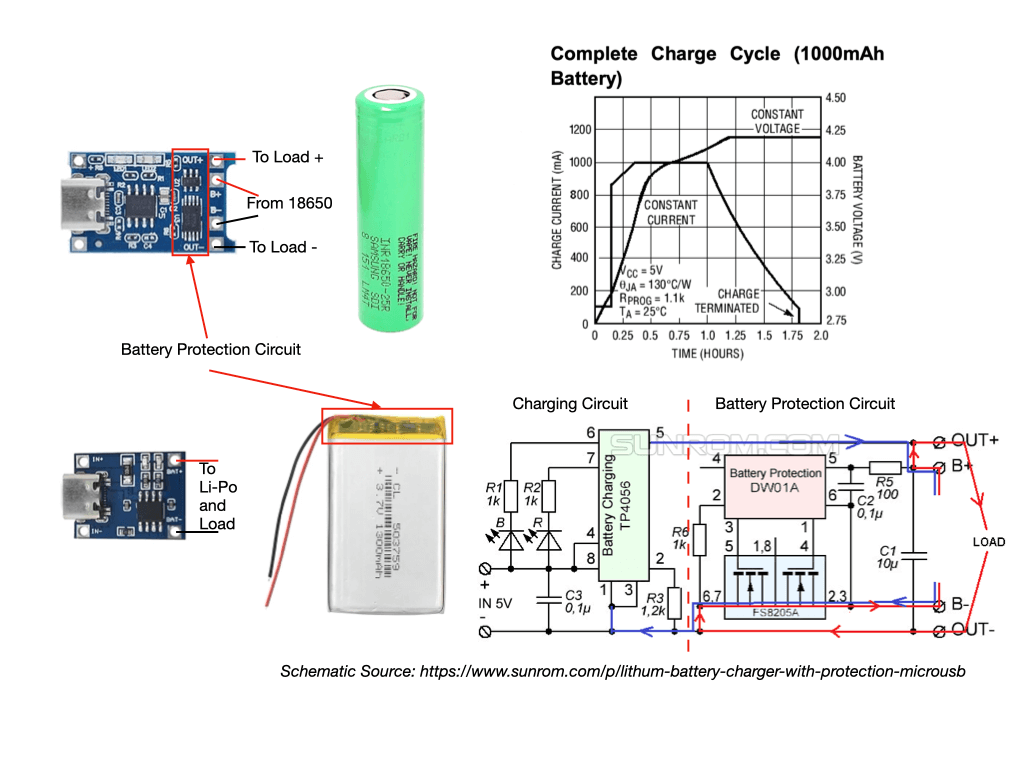
\includegraphics[width=0.8\textwidth]{photos/battery_protection_circuit.png}
%     \caption{Ochrana baterie}
%     \label{fig:graf_podslozka}
% \end{figure}


% --------------------------------------------------
% --------------------------------------------------

\section{SOFTWARE}
% https://www.phippselectronics.com/how-to-play-a-wav-file-on-stm32/


% - WAV soubor je založen na kontejneru RIFF = Resource Interchange File 

% - RIFF se skládá z menších bloků, "chunks", každý chunk má čtyřznakový identifikátor FOURCC

% \begin{itemize}
%     \item ChunkID, File offset 0, velikost 4 B, 0x52494646 (v ASCII "RIFF"), big endian
%     \item ChunkSize, File offset 4, velikost 4 B
%     \item Format, File offset 8, velikost 4 B, 0x57415645 (v ASCII "WAVE")
% \end{itemize}

% Následuje "FMT" sub-chunk,
% \begin{itemize}
%     \item Subchunk1ID, obsahuje 4 B dat jako 0x666d420. 66 = "f", 6d = "m", 74 = "t" 20 = mezera, space
%     \item SubchunkSize, 16 pro PCM (0x10000000). Určuje velikost zbytku subchunku.
%     \item AudioFormat, 1 pro PCM (linear quantization), pokud je zde jiné číslo než 1, jde o kompresi
%     \item NumChannels, Mono = 1, Stereo = 2 (velikost 2B)
%     \item SampleRate, např. 48000 (velikost 4B)
%     \item ByteRate = SampleRate * NumChannels * BitsPerSample/8
%     \item BlockAlign = NumChannels * BitsPerSample/8
%     \item BitsPerSample, 8 bits = 8, 16 bits = 16
% \end{itemize}

% A za ním pak "data" subchunk, obsahující počet bajtů v "data" a samotný zvuk.
% \begin{itemize}
%     \item Subchunk2ID, 4 B dat, 0x64617461. 64 = "d", 61 = "a", 74 = "t", 61 = "a"
%     \item Subchunk2Size
%     \item Data

% \end{itemize}

\subsection{Formát souboru WAV}

Formát WAV (\textit{Waveform Audio File Format}) je založen na kontejnerovém
formátu RIFF (\textit{Resource Interchange File Format}). Soubor ve formátu
RIFF se skládá z jednotlivých bloků označovaných jako \textit{chunks}.
Každý blok je identifikován čtyřznakovým identifikátorem FOURCC
(\textit{Four-Character Code}).

V případě běžného nekomprimovaného PCM WAV souboru se struktura skládá
z hlavičky RIFF a následných bloků \texttt{fmt} a \texttt{data}.
Zde je základní struktura hlavičky RIFF:
\ref{tab:wav_riff_header}.

\begin{table}[ht]
    \centering
    \caption{Struktura hlavičky RIFF souboru WAV}
    \label{tab:wav_riff_header}
    \begin{tabular}{lccc}
        \toprule
        \textbf{Pole} & \textbf{Offset [B]} & \textbf{Velikost [B]} & \textbf{Význam} \\
        \midrule
        \texttt{ChunkID}   & 0 & 4 & ASCII řetězec \texttt{RIFF} \\
        \texttt{ChunkSize} & 4 & 4 & Velikost souboru bez prvních 8 bajtů \\
        \texttt{Format}    & 8 & 4 & ASCII řetězec \texttt{WAVE} \\
        \bottomrule
    \end{tabular}
\end{table}

Pole \texttt{ChunkID} obsahuje posloupnost znaků \texttt{RIFF}, odpovídající bajtům \texttt{52 49 46 46}. Pole \texttt{ChunkSize}
udává velikost zbývající části RIFF bloku, tedy v případě základního
WAV souboru velikost celého souboru zmenšenou o 8 bajtů. Pole
\texttt{Format} obsahuje identifikátor \texttt{WAVE}.

Za hlavičkou RIFF následuje blok \texttt{fmt}, popisující formát uložených zvukových dat. Jeho struktura pro nekomprimovaný PCM signál je uvedena v tabulce \ref{tab:wav_fmt}.

\begin{table}[ht]
    \centering
    \caption{Struktura bloku \texttt{fmt } pro PCM WAV}
    \label{tab:wav_fmt}
    \begin{tabular}{lccp{7cm}}
        \toprule
        \textbf{Pole} & \textbf{Offset [B]} & \textbf{Velikost [B]} & \textbf{Význam} \\
        \midrule
        \texttt{Subchunk1ID}
        & 12 & 4
        & ASCII řetězec \texttt{fmt } \\

        \texttt{Subchunk1Size}
        & 16 & 4
        & Velikost zbývající části bloku; pro PCM je rovna 16 B \\

        \texttt{AudioFormat}
        & 20 & 2
        & Formát zvukových dat; hodnota 1 označuje PCM \\

        \texttt{NumChannels}
        & 22 & 2
        & Počet zvukových kanálů; 1 pro mono, 2 pro stereo \\

        \texttt{SampleRate}
        & 24 & 4
        & Vzorkovací frekvence v Hz, například 48\,000 Hz \\

        \texttt{ByteRate}
        & 28 & 4
        & Počet bajtů za sekundu \\

        \texttt{BlockAlign}
        & 32 & 2
        & Počet bajtů jednoho vzorkovacího rámce \\

        \texttt{BitsPerSample}
        & 34 & 2
        & Bitová hloubka jednoho vzorku \\
        \bottomrule
    \end{tabular}
\end{table}

Hodnota pole \texttt{ByteRate} je určena vztahem

\begin{equation}
    \texttt{ByteRate}
    =
    \texttt{SampleRate}
    \cdot
    \texttt{NumChannels}
    \cdot
    \frac{\texttt{BitsPerSample}}{8}.
\end{equation}

Podobně lze velikost jednoho vzorkovacího rámce vyjádřit jako

\begin{equation}
    \texttt{BlockAlign}
    =
    \texttt{NumChannels}
    \cdot
    \frac{\texttt{BitsPerSample}}{8}.
\end{equation}

Vzorkovací rámec zde představuje vzorky všech kanálů náležející ke
stejnému okamžiku vzorkování. Například u 16bitového stereofonního
signálu má jeden rámec velikost 4 B.

Za blokem \texttt{fmt } se v základní podobě PCM WAV souboru nachází
blok \texttt{data}, který obsahuje vlastní zvuková data.

\begin{table}[ht]
    \centering
    \caption{Struktura bloku \texttt{data}}
    \label{tab:wav_data}
    \begin{tabular}{lccp{7cm}}
        \toprule
        \textbf{Pole} & \textbf{Offset [B]} & \textbf{Velikost [B]} & \textbf{Význam} \\
        \midrule
        \texttt{Subchunk2ID}
        & 36 & 4
        & ASCII řetězec \texttt{data} \\

        \texttt{Subchunk2Size}
        & 40 & 4
        & Počet bajtů zvukových dat \\

        \texttt{Data}
        & 44 & proměnná
        & Jednotlivé vzorky zvukového signálu \\
        \bottomrule
    \end{tabular}
\end{table}

Velikost datové části lze pro PCM signál vyjádřit jako

\begin{equation}
    \texttt{Subchunk2Size}
    =
    N_\mathrm{samples}
    \cdot
    \texttt{NumChannels}
    \cdot
    \frac{\texttt{BitsPerSample}}{8},
\end{equation}

kde $N_\mathrm{samples}$ představuje počet vzorků jednoho kanálu.

Vícebajtové číselné hodnoty jsou ve standardním WAV souboru ukládány v pořadí \textit{little-endian}. Například 32bitová hodnota \texttt{0x12345678} je tedy v souboru uložena jako posloupnost bajtů \texttt{78 56 34 12}. Čtyřznakové identifikátory, například \texttt{RIFF}, \texttt{WAVE}, \texttt{fmt } nebo \texttt{data}, jsou naproti tomu ukládány přímo jako posloupnost ASCII znaků\cite{wav_internet_archive}.

\subsubsection{Načítání WAV do STM32}
https://www.phippselectronics.com/how-to-play-a-wav-file-on-stm32/
% --------------------------------------------------
% --------------------------------------------------



\printbibliography
\end{document}
